\chapter{Methods}\label{ch:expt}


\section{Substrate preparation}

This is a good chapter to write continuously throughout your degree program.  It will be easier to write up a procedure while it's fresh in your mind, and that way you won't be hunting down an instrument model or consumables supplier later.

If you are varying several parameters in your procedure, you may want to tabulate your different combinations.  Table \ref{icecream} summarizes ice cream texture characteristics used by McGhee et al\cite{McGhee}.

\begin{table}[!htbp]
\caption[Note how this caption is at the top of the table.  Also, note that the caption in the List of Tables doesn't include the reference number.]{Note how this caption is at the top of the table.  Also, note that the caption in the List of Tables doesn't include the reference number.\cite{McGhee}. \label{icecream}}

\centering
\begin{tabular}{lc}
 Characteristic& Mean value\\\hline
Icy	 &4.63\\
Crumbly	 &4.75\\
Fluffy	 &4.58\\
Gummy	 &4.71\\
Sandy	 &4.58\\
Soggy	 &4.29\\
Weak body&3.92\\
\end{tabular}
\end{table}

\subsection{Lots of chemicals}

I used \ce{K2HPO4}, \ce{KH2PO4.2H2O}, and other salts containing \ce{PO4^{3-}} ions.  Best of all, I didn't write out those chemical formula by hand using subscripts and superscripts.  See the .tex file to find out how!

\section{Atomic Force Microscopy}

A picture is worth a thousand words!  If you are creating your own schematics, consider using a program which will saves images in a precise and generally readable format such as SVG.  Inkscape will do that for you and is open source.

There are many public domain and other freely reproducible images available on the Wikimedia Commons.  You can also easily get permission to reuse a figure from most journals through RightsLink.

\begin{figure}[!hbtp]
\centering
    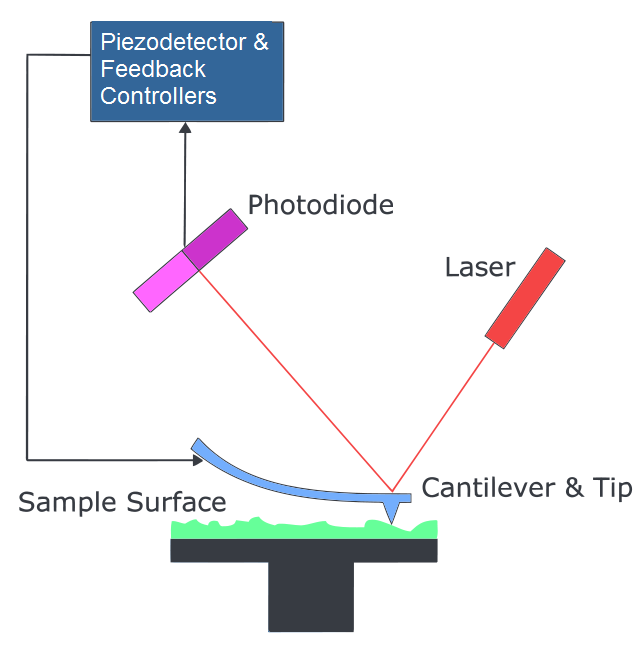
\includegraphics[totalheight=0.5\textwidth, natwidth=640,natheight=640]{640px-Atomic_force_microscope_block_diagram.png}
\caption{Schematic of an atomic force microscope. Note that the size of the text in the figure is comparable to the size of the main text.  Reproduced under Public Domain from Wikimedia Commons\label{AFMblock}}
\end{figure} 


